\documentclass[10pt]{article}
\usepackage[a4paper,margin=15mm]{geometry}
\usepackage[T1]{fontenc}
\usepackage[utf8]{inputenc}
\usepackage{lmodern}
\usepackage{xcolor}
\usepackage{tikz}
\usetikzlibrary{arrows.meta,positioning,fit,calc,shapes.geometric}
\usepackage[most]{tcolorbox}
\usepackage{listings}
\usepackage{amsmath,amssymb}
\usepackage{microtype}
\usepackage{enumitem}
\usepackage[hidelinks]{hyperref}
\pagestyle{empty}

\definecolor{ink}{HTML}{23313A}
\definecolor{muted}{HTML}{62727B}
\definecolor{blue}{HTML}{286BE6}
\definecolor{bluepale}{HTML}{EDF3FF}
\definecolor{teal}{HTML}{108A7A}
\definecolor{tealpale}{HTML}{E8F7F3}
\definecolor{amber}{HTML}{C97B0A}
\definecolor{amberpale}{HTML}{FFF3DD}
\definecolor{red}{HTML}{C84B4B}
\definecolor{redpale}{HTML}{FFF0F0}
\definecolor{line}{HTML}{D8E2E7}
\definecolor{codebg}{HTML}{F6F8FA}

\color{ink}
\setlength{\parindent}{0pt}
\setlength{\parskip}{3pt}
\setlist{nosep,leftmargin=1.3em}
\newcommand{\pill}[2]{\tikz[baseline=(x.base)]\node[rounded corners=3pt,fill=#1,inner xsep=5pt,inner ysep=2pt,text=ink,font=\sffamily\scriptsize\bfseries] (x) {#2};}
\newcommand{\sect}[1]{\vspace{2pt}{\sffamily\bfseries\large #1}\par\vspace{4pt}}
\newcommand{\leanname}[1]{\texttt{#1}}

\lstdefinelanguage{Lean}{
  morekeywords={theorem,lemma,where,by,apply,exact,obtain,rintro,fun,cases,with,let,in,if,then,else},
  morekeywords=[2]{Type,Sort,CompleteSemilatticeSup,Set,ENat,ENNReal},
  morecomment=[l]{--},morecomment=[s]{/-}{-/},sensitive=true
}
\lstset{language=Lean,basicstyle=\ttfamily\fontsize{7.25}{8.7}\selectfont,
  keywordstyle=\color{blue}\bfseries,keywordstyle=[2]\color{teal},
  commentstyle=\color{muted}\itshape,showstringspaces=false,
  columns=fullflexible,keepspaces=true,aboveskip=3pt,belowskip=2pt}
\newtcolorbox{softbox}[2][]{enhanced,boxrule=.6pt,arc=5pt,colback=#2,colframe=line,
  left=8pt,right=8pt,top=6pt,bottom=6pt,#1}
\tikzset{
  card/.style={draw=line,rounded corners=5pt,align=left,inner sep=7pt,font=\sffamily\small},
  arr/.style={-{Latex[length=2.3mm]},very thick,color=muted},
  thinarr/.style={-{Latex[length=2mm]},thick,color=muted}
}

\begin{document}

% PAGINA 1
{\sffamily\fontsize{22}{25}\selectfont\bfseries Dalle prove duplicate a un lemma riusabile}\par
\vspace{3pt}
{\sffamily\color{muted}Visualizzazione del pattern e dell'idea matematica}\hfill
\pill{bluepale}{RIPETIZIONE}\;\pill{tealpale}{ASTRAZIONE}\;\pill{amberpale}{RIUSO}

\vspace{12pt}
\begin{center}
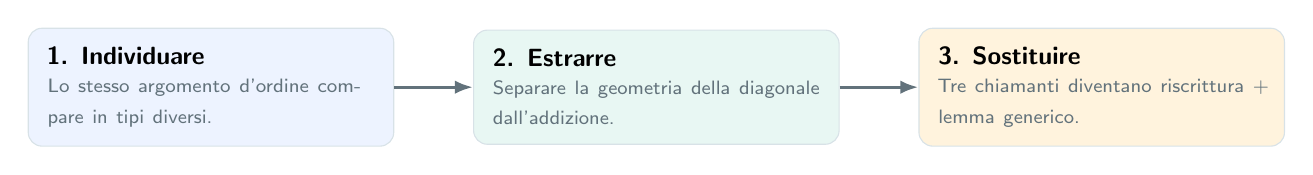
\begin{tikzpicture}[node distance=8mm and 10mm]
  \node[card,fill=bluepale,text width=4.15cm,minimum height=1.2cm] (a)
    {\textbf{1. Individuare}\\[-1pt]\scriptsize\color{muted}Lo stesso argomento d'ordine compare in tipi diversi.};
  \node[card,fill=tealpale,text width=4.15cm,minimum height=1.2cm,right=of a] (b)
    {\textbf{2. Estrarre}\\[-1pt]\scriptsize\color{muted}Separare la geometria della diagonale dall'addizione.};
  \node[card,fill=amberpale,text width=4.15cm,minimum height=1.2cm,right=of b] (c)
    {\textbf{3. Sostituire}\\[-1pt]\scriptsize\color{muted}Tre chiamanti diventano riscrittura + lemma generico.};
  \draw[arr] (a)--(b); \draw[arr] (b)--(c);
\end{tikzpicture}
\end{center}

\vspace{7pt}
\sect{La forma duplicata osservata}
\begin{softbox}{codebg}
\begin{minipage}[t]{.48\linewidth}
\pill{bluepale}{ENat.iSup\_add\_iSup}
\begin{lstlisting}
refine le_antisymm ?_ ?_
refine iSup_add_iSup_le fun i j => ?_
rcases h i j with <k, hk>
exact le_iSup_of_le k hk
\end{lstlisting}
\end{minipage}\hfill
\begin{minipage}[t]{.48\linewidth}
\pill{bluepale}{ENNReal.iSup\_add\_iSup}
\begin{lstlisting}
refine le_antisymm ?_ ?_
refine iSup_add_iSup_le fun i j => ?_
rcases h i j with <k, hk>
exact le_iSup_of_le k hk
\end{lstlisting}
\end{minipage}
\end{softbox}

\vspace{7pt}
\sect{L'invariante: la diagonale è cofinale}
\begin{center}
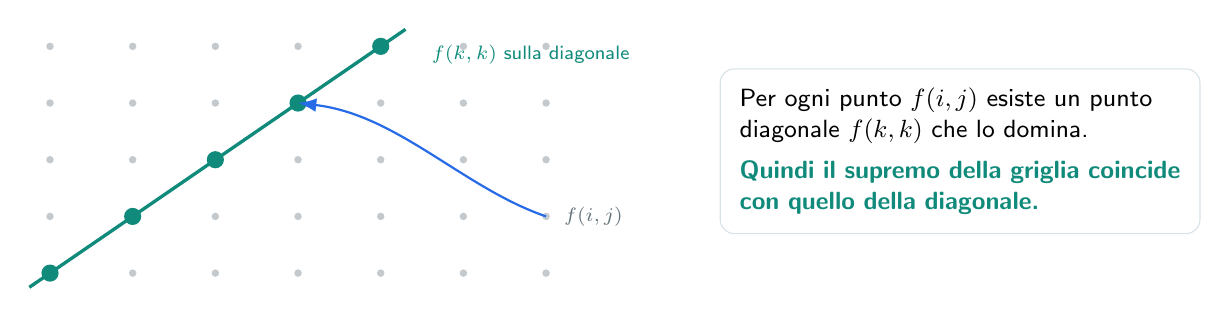
\begin{tikzpicture}[x=1.05cm,y=.72cm]
  \foreach \x in {0,...,6} {\foreach \y in {0,...,4} {\fill[muted!38] (\x,\y) circle (1.35pt);}}
  \foreach \k in {0,...,4} {\fill[teal] (\k,\k) circle (3.1pt);}
  \draw[teal,very thick] (-.25,-.25)--(4.3,4.3);
  \draw[blue,-{Latex},thick] (6,1) .. controls (5.0,1.5) and (4.2,2.8) .. (3,3);
  \node[font=\sffamily\scriptsize,text=muted,anchor=west] at (6.1,1) {$f(i,j)$};
  \node[font=\sffamily\scriptsize,text=teal,anchor=west] at (4.5,3.85) {$f(k,k)$ sulla diagonale};
  \node[card,fill=white,text width=5.6cm,anchor=west] at (8.1,2.15)
    {Per ogni punto $f(i,j)$ esiste un punto diagonale $f(k,k)$ che lo domina.\\[4pt]
     \color{teal}\bfseries Quindi il supremo della griglia coincide con quello della diagonale.};
\end{tikzpicture}
\end{center}

\vspace{6pt}
\begin{softbox}{tealpale}
\centering
$\displaystyle \bigvee_i\bigvee_j f(i,j)=\bigvee_k f(k,k)$
\qquad se \qquad
$\displaystyle \forall i,j\;\exists k,\ f(i,j)\le f(k,k)$.
\end{softbox}

\vfill
{\color{muted}\scriptsize\sffamily Idea guida: astrarre la struttura d'ordine comune, non l'operazione specifica dei chiamanti.}

\newpage

% PAGINA 2
{\sffamily\fontsize{22}{25}\selectfont\bfseries Tre livelli di generalità}\par
\vspace{3pt}
{\sffamily\color{muted}Dal caso applicativo al possibile lemma strutturale}\hfill\pill{tealpale}{BIG IDEA}

\vspace{12pt}
\begin{center}
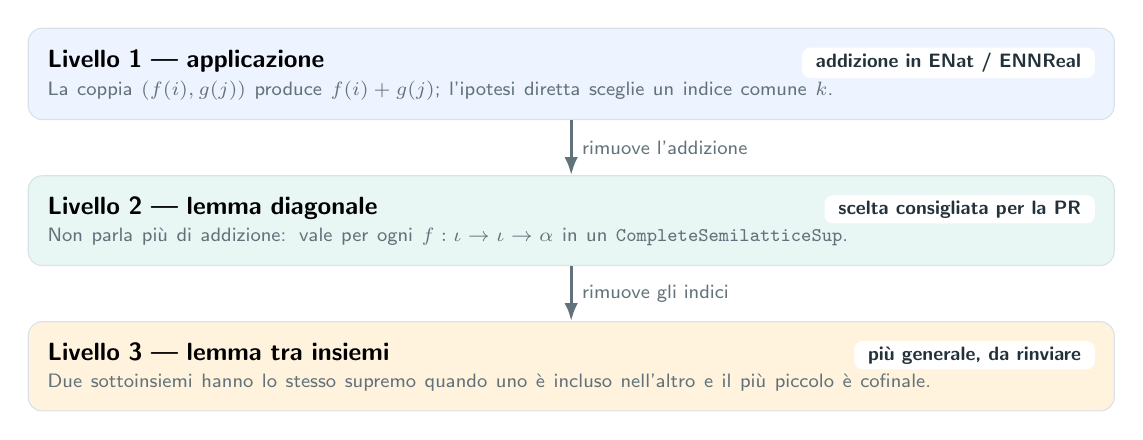
\begin{tikzpicture}[node distance=7mm]
  \node[card,fill=bluepale,text width=13.3cm] (l1)
    {\textbf{Livello 1 --- applicazione}\hfill\pill{white}{addizione in ENat / ENNReal}\\[-1pt]
     \scriptsize\color{muted}La coppia $(f(i),g(j))$ produce $f(i)+g(j)$; l'ipotesi diretta sceglie un indice comune $k$.};
  \node[card,fill=tealpale,text width=13.3cm,below=of l1] (l2)
    {\textbf{Livello 2 --- lemma diagonale}\hfill\pill{white}{scelta consigliata per la PR}\\[-1pt]
     \scriptsize\color{muted}Non parla più di addizione: vale per ogni $f:\iota\to\iota\to\alpha$ in un \texttt{CompleteSemilatticeSup}.};
  \node[card,fill=amberpale,text width=13.3cm,below=of l2] (l3)
    {\textbf{Livello 3 --- lemma tra insiemi}\hfill\pill{white}{più generale, da rinviare}\\[-1pt]
     \scriptsize\color{muted}Due sottoinsiemi hanno lo stesso supremo quando uno è incluso nell'altro e il più piccolo è cofinale.};
  \draw[arr] (l1)--node[right,font=\sffamily\scriptsize,text=muted]{rimuove l'addizione} (l2);
  \draw[arr] (l2)--node[right,font=\sffamily\scriptsize,text=muted]{rimuove gli indici} (l3);
\end{tikzpicture}
\end{center}

\vspace{8pt}
\sect{Il lemma da proporre ora}
\begin{softbox}{tealpale}
\begin{lstlisting}
@[to_dual iInf2_eq_diagonal]
theorem iSup2_eq_diagonal
    [CompleteSemilatticeSup alpha] (f : iota -> iota -> alpha)
    (h : forall i j, exists k, f i j <= f k k) :
    (iSup i, iSup j, f i j) = iSup k, f k k := by
  ...
\end{lstlisting}
\end{softbox}

\vspace{7pt}
\begin{center}
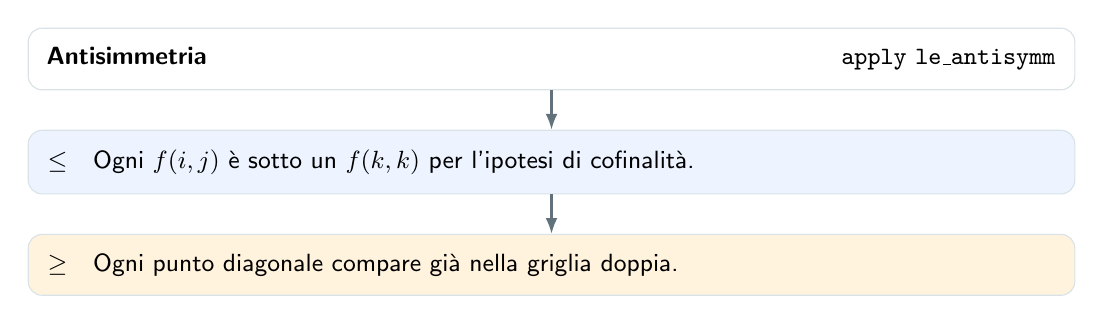
\begin{tikzpicture}[node distance=5mm]
  \node[card,fill=white,text width=12.8cm] (p0) {\textbf{Antisimmetria}\hfill\texttt{apply le\_antisymm}};
  \node[card,fill=bluepale,text width=12.8cm,below=of p0] (p1) {\textbf{$\le$}\quad Ogni $f(i,j)$ è sotto un $f(k,k)$ per l'ipotesi di cofinalità.};
  \node[card,fill=amberpale,text width=12.8cm,below=of p1] (p2) {\textbf{$\ge$}\quad Ogni punto diagonale compare già nella griglia doppia.};
  \draw[thinarr] (p0)--(p1); \draw[thinarr] (p1)--(p2);
\end{tikzpicture}
\end{center}

\vspace{8pt}
\sect{Il lemma ancora più generale}
\begin{softbox}{amberpale}
\begin{lstlisting}
theorem sSup_eq_sSup_of_subset_of_isCofinalFor
    [CompleteSemilatticeSup alpha] {s t : Set alpha}
    (hst : s subset t) (hts : IsCofinalFor t s) :
    sSup s = sSup t := by
  apply le_antisymm
  . exact sSup_le_sSup hst
  . exact sSup_le_sSup_of_isCofinalFor hts
\end{lstlisting}
\end{softbox}

\begin{center}
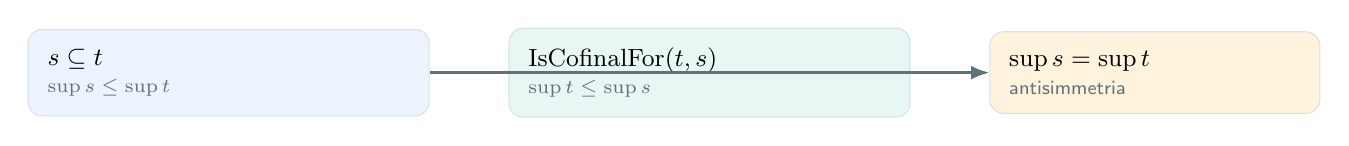
\begin{tikzpicture}[node distance=7mm and 10mm]
  \node[card,fill=bluepale,text width=4.6cm] (a) {$s\subseteq t$\\[-1pt]\scriptsize\color{muted}$\sup s\le\sup t$};
  \node[card,fill=tealpale,text width=4.6cm,right=of a] (b) {$\mathrm{IsCofinalFor}(t,s)$\\[-1pt]\scriptsize\color{muted}$\sup t\le\sup s$};
  \node[card,fill=amberpale,text width=3.7cm,right=of b] (c) {$\sup s=\sup t$\\[-1pt]\scriptsize\color{muted}antisimmetria};
  \draw[arr] (a)--(c); \draw[arr] (b)--(c);
\end{tikzpicture}
\end{center}

\vfill
{\color{muted}\scriptsize\sffamily Nota API: l'orientamento corretto è \texttt{IsCofinalFor t s}; il lemma disponibile è \texttt{sSup\_le\_sSup}.}

\newpage

% PAGINA 3
{\sffamily\fontsize{22}{25}\selectfont\bfseries Cosa mettere nella PR}\par
\vspace{3pt}
{\sffamily\color{muted}Una decisione basata su riuso dimostrato e costo di revisione}\hfill\pill{amberpale}{PR PLAN}

\vspace{12pt}
\begin{center}
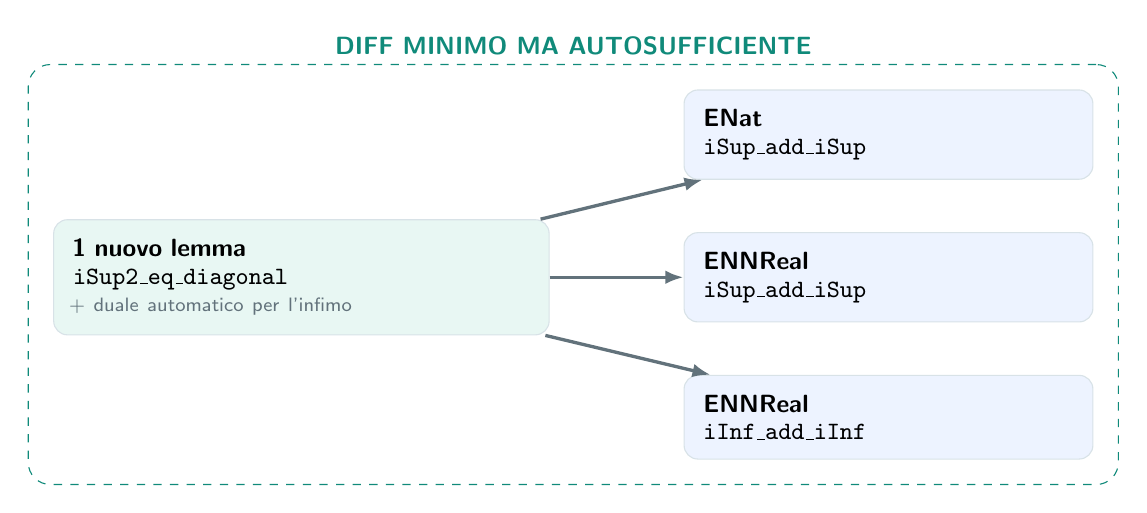
\begin{tikzpicture}[node distance=8mm and 13mm]
  \node[card,fill=tealpale,text width=5.8cm,minimum height=1.3cm] (core)
    {\textbf{1 nuovo lemma}\\[-1pt]\texttt{iSup2\_eq\_diagonal}\\[-1pt]\scriptsize\color{muted}+ duale automatico per l'infimo};
  \node[card,fill=bluepale,text width=4.7cm,above right=5mm and 17mm of core] (e1)
    {\textbf{ENat}\\[-1pt]\texttt{iSup\_add\_iSup}};
  \node[card,fill=bluepale,text width=4.7cm,right=17mm of core] (e2)
    {\textbf{ENNReal}\\[-1pt]\texttt{iSup\_add\_iSup}};
  \node[card,fill=bluepale,text width=4.7cm,below right=5mm and 17mm of core] (e3)
    {\textbf{ENNReal}\\[-1pt]\texttt{iInf\_add\_iInf}};
  \draw[arr] (core)--(e1); \draw[arr] (core)--(e2); \draw[arr] (core)--(e3);
  \node[draw=teal,dashed,rounded corners=8pt,fit=(core)(e1)(e2)(e3),inner sep=9pt,
    label={[font=\sffamily\small\bfseries,text=teal]above:DIFF MINIMO MA AUTOSUFFICIENTE}] {};
\end{tikzpicture}
\end{center}

\vspace{12pt}
\begin{minipage}[t]{.485\linewidth}
\begin{softbox}{tealpale}
{\sffamily\bfseries Includere}\par
\begin{itemize}
  \item il lemma in \texttt{Order/CompleteLattice/}\\\texttt{Basic.lean};
  \item classe minima\\\texttt{CompleteSemilatticeSup};
  \item dualità: \texttt{@[to\_dual}\\\texttt{iInf2\_eq\_diagonal]};
  \item i tre refactor sopra;
  \item docstring breve: ``diagonale cofinale'';
  \item build, lint e test della patch.
\end{itemize}
\end{softbox}
\end{minipage}\hfill
\begin{minipage}[t]{.485\linewidth}
\begin{softbox}{redpale}
{\sffamily\bfseries Non includere nella prima PR}\par
\begin{itemize}
  \item il wrapper generale su \texttt{sSup};
  \item varianti condizionalmente complete;
  \item refactor del caso \texttt{Cardinal};
  \item nuovi framework o molte varianti stilistiche;
  \item modifiche al workflow CI non collegate.
\end{itemize}
\end{softbox}
\end{minipage}

\vspace{10pt}
\sect{Lasciare la PR così o migliorarla?}
\begin{center}
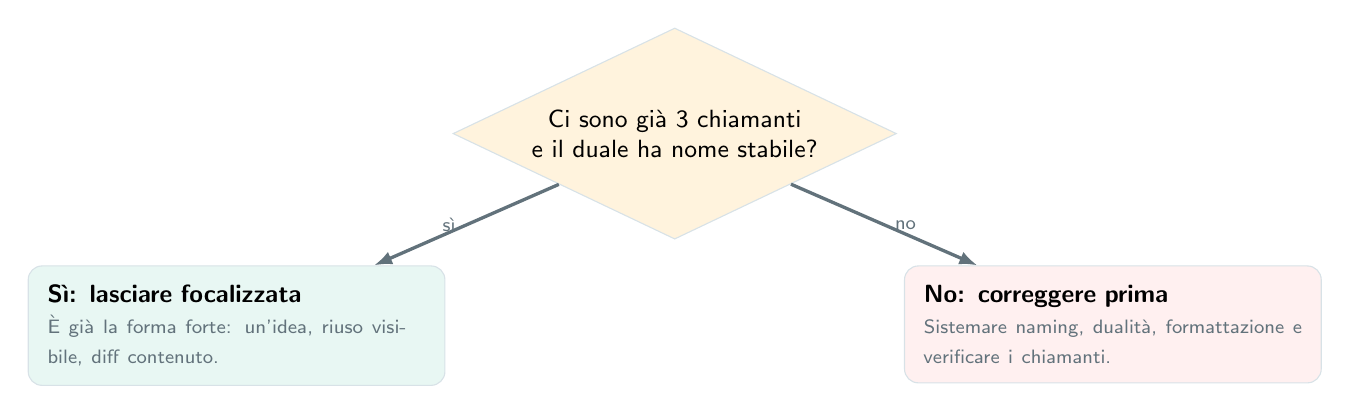
\begin{tikzpicture}[node distance=7mm and 10mm]
  \node[diamond,draw=line,fill=amberpale,aspect=2.1,align=center,font=\sffamily\small] (q)
    {Ci sono già 3 chiamanti\\e il duale ha nome stabile?};
  \node[card,fill=tealpale,text width=4.8cm,below left=10mm and 15mm of q] (yes)
    {\textbf{Sì: lasciare focalizzata}\par\scriptsize\color{muted}È già la forma forte: un'idea, riuso visibile, diff contenuto.};
  \node[card,fill=redpale,text width=4.8cm,below right=10mm and 15mm of q] (no)
    {\textbf{No: correggere prima}\par\scriptsize\color{muted}Sistemare naming, dualità, formattazione e verificare i chiamanti.};
  \draw[arr] (q)--node[left,font=\sffamily\scriptsize]{sì} (yes);
  \draw[arr] (q)--node[right,font=\sffamily\scriptsize]{no} (no);
\end{tikzpicture}
\end{center}

\vspace{8pt}
\begin{softbox}{bluepale}
{\sffamily\bfseries Miglioramento consigliato del testo della PR}\par
\small
``Tre prove implementavano lo stesso fatto d'ordine: una diagonale cofinale ha lo stesso supremo
della famiglia doppiamente indicizzata. Questa PR estrae il risultato sotto
\texttt{CompleteSemilatticeSup}, genera il duale e semplifica i tre chiamanti esistenti.''
\end{softbox}

\vspace{8pt}
\begin{softbox}{amberpale}
{\sffamily\bfseries Quando aprire un seguito sul lemma generale}\par
Solo dopo aver trovato un secondo uso indipendente di
\texttt{sSup\_eq\_sSup\_of\_subset\_of\_isCofinalFor}, oppure se un reviewer chiede
esplicitamente di organizzare l'API attorno a \texttt{IsCofinalFor}.
\end{softbox}

\vfill
{\color{muted}\scriptsize\sffamily Raccomandazione finale: PR corrente = lemma diagonale + duale + tre chiamanti. Il wrapper su \texttt{sSup} resta una proposta separata.}

\end{document}
